% Level 3 workbook, Week 12 -- Showcase and Graduation
\chapterweek{12}{Showcase and Graduation}{Share what you built, explain your choices, and plan what comes next.}

\section{What you will do}
\begin{itemize}[itemsep=1pt]
  \item Give a \textbf{2-minute design talk} about one decision in your project.
  \item Visit everyone's project in a \textbf{gallery walk} and give helpful feedback.
  \item Show what you have learned in the \textbf{exit assessment}.
  \item Look back at your journey and plan your \textbf{next steps}, safely.
\end{itemize}

\section{The big idea: explain the \emph{why}}
Anyone can say \emph{what} their program does. A real developer can explain \emph{why} they built it that way. In two minutes, pick \textbf{one} decision and walk through four steps:

\begin{center}
%% alt: Four steps for explaining a design decision. 1 Problem: what was hard or not working? 2 Choice: what did you decide to do? 3 Why: why that way and not another? 4 Next time: what would you change?
\begin{tikzpicture}[st/.style={draw,thick,rounded corners=3pt,minimum width=3.3cm,minimum height=1.5cm,align=center,font=\small},>=Stealth]
  \node[st,fill=kcorange!20] (p) at (0,0) {\textbf{1 Problem}\\What was hard\\or not working?};
  \node[st,fill=kcsky!20] (c) at (3.9,0) {\textbf{2 Choice}\\What did you\\decide to do?};
  \node[st,fill=kcgreen!20] (w) at (7.8,0) {\textbf{3 Why}\\Why that way\\and not another?};
  \node[st,fill=kcpurple!20] (n) at (11.7,0) {\textbf{4 Next time}\\What would\\you change?};
  \draw[->,thick] (p) -- (c); \draw[->,thick] (c) -- (w); \draw[->,thick] (w) -- (n);
\end{tikzpicture}
\end{center}

\textbf{Example:} \enquote{\textbf{Problem:} my first ghost moved randomly and the game was too easy. \textbf{Choice:} I made a Chaser class that \emph{is a} Ghost, and its move uses breadth-first search with a queue. \textbf{Why:} inheritance meant I only wrote the new part, and BFS always finds the shortest path. \textbf{Next time:} the Chaser is too clever -- it should only chase every other turn.}

Good decisions to talk about: why you chose inheritance or composition, why a dictionary or a grid, which algorithm and why, what a test caught, what a playtester taught you.

\begin{exercise}[My showcase talk card]
\begin{tabular}{@{}p{3.2cm}p{\dimexpr\linewidth-3.4cm-2\tabcolsep}@{}}
My project in one sentence: & \rule{\linewidth}{0.4pt}\\[8pt]
1 Problem: & \rule{\linewidth}{0.4pt}\\[8pt]
2 Choice: & \rule{\linewidth}{0.4pt}\\[8pt]
3 Why: & \rule{\linewidth}{0.4pt}\\[8pt]
4 Next time: & \rule{\linewidth}{0.4pt}\\[8pt]
What I will show: & $\square$ playing it \quad $\square$ a class \quad $\square$ a test \quad $\square$ \texttt{git log}\\
\end{tabular}
\end{exercise}

\section{Gallery walk: star and wish}
Feedback helps when it is \textbf{kind}, \textbf{specific} and \textbf{useful}. \enquote{Cool!} is kind but not useful. \enquote{The score text was big and easy to read} is all three.

\begin{exercise}[Feedback cards]
Write one card for each project you visit. Leave it face down next to the computer.
\begin{center}
%% alt: Four blank feedback cards, each with a line for the project name and spaces for a Star (I liked…) and a Wish (What if…?).
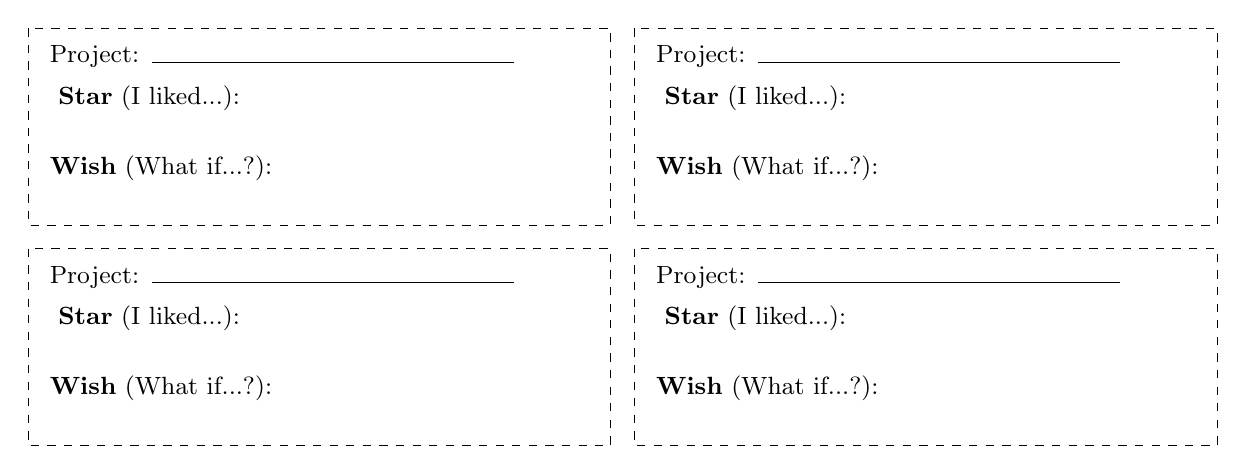
\begin{tikzpicture}
  \foreach \x/\y in {0/0,7.7/0,0/-2.8,7.7/-2.8}{
    \draw[dashed] (\x,\y) rectangle ++(7.4,-2.5);
    \node[anchor=north west,font=\small,text width=7cm] at (\x+0.15,\y-0.1) {Project: \rule{4.6cm}{0.4pt}\\[4pt]$\bigstar$ \textbf{Star} (I liked...):\\[0.5cm]\textbf{Wish} (What if...?):};
  }
\end{tikzpicture}
\end{center}
\end{exercise}

\section{Look how far you have come}
\begin{center}
%% alt: A timeline of the level: week 1 git save points, weeks 2 and 3 classes and objects, weeks 4 and 5 search and sort, week 7 recursion and grids, weeks 8 and 9 data and AI, and weeks 10 to 12 my big project.
\begin{tikzpicture}[m/.style={draw,rounded corners=2pt,fill=kcyellow!20,font=\small,align=center,minimum width=2.2cm,minimum height=1cm},>=Stealth]
  \draw[thick,->] (-0.5,0) -- (15.6,0);
  \foreach \x/\t/\w in {0.7/{git\\save points}/1, 3.2/{classes \&\\objects}/2--3, 5.7/{search \&\\sort}/4--5, 8.2/{recursion\\\& grids}/7, 10.7/{data \&\\AI}/8--9, 13.4/{my big\\project}/10--12}{
    \node[m] at (\x,0.95) {\t};
    \fill (\x,0) circle (2pt);
    \node[below,font=\scriptsize] at (\x,-0.1) {week \w};
  }
\end{tikzpicture}
\end{center}

\begin{exercise}[My Level 3 journey]
Run \texttt{git log --oneline} in your project. How many commits? \rule{1.5cm}{0.4pt}
The skill I am proudest of: \answerlines{1}
Something that was hard at first and is easier now: \answerlines{1}
\end{exercise}

\section{What next? Keep coding, safely}
You can keep learning on your own. Some ideas: give your project a version 2; learn another Python library with a parent's help; try a new kind of program (a text adventure, a simulation, a puzzle solver); teach someone younger what you know.

\begin{safety}[Next steps online]
If you want to share your work or join a coding community, \textbf{choose it together with a parent}. Look for clear rules, moderators and a code of conduct. Use a \textbf{nickname} -- never your real name, school, age, face or location, in the project or the account. Never move to private chats with strangers, never send photos, and tell an adult straight away if anything feels wrong. Your projects are yours: share only what you want to share.
\end{safety}

\begin{vocab}
  \vocabword{design decision}{A choice about how to build something, with a reason.}
  \vocabword{feedback}{Comments that help someone improve: kind, specific, useful.}
  \vocabword{showcase}{An event where makers show and explain their work.}
  \vocabword{code of conduct}{The rules a community agrees to, so everyone stays safe and respected.}
  \vocabword{version 2}{The next, improved release of a project.}
\end{vocab}

\begin{reflection}
Which feedback card made you proudest? \answerlines{1}
What will you build next? \answerlines{2}
\end{reflection}
